\documentclass[conference]{acmsiggraph}

\usepackage{mdwlist}
\usepackage{graphics}
\usepackage{graphicx}
\usepackage{listings}
\usepackage{enumitem}

%%%%%%%%%%%%%%%
% Information %
%%%%%%%%%%%%%%%

\title{Plant Modeling Using Environmental Parameters}

\author{
  Andre Philipp\thanks{e-mail:philipp.andy@gmail.com}
  \qquad
  Andy Spencer\thanks{e-mail:e-mail:andy753421@ucla.edu}
  \qquad
  Haakon Garseg Mørk\thanks{e-mail:haakongmork@gmail.com}
  \\
  University of California, Los Angeles \\
  CS275 Artificial Life for Computer Graphics and Vision
}


\pdfauthor{Andre Philipp, Andy Spencer, Haakon Garseg Mørk}

\keywords{radiosity, global illumination, constant time}

%%%%%%%%%%%%
% Document %
%%%%%%%%%%%%

\begin{document}

%%%%%%%%%%%%%%
% Title Page %
%%%%%%%%%%%%%%

\maketitle

\begin{abstract}

The project will focus on modeling natural looking plants using simulated
environment parameters to control growth and evolution of different plant
species. Genetic algorithms or other evolutionary techniques will be used to
evolve plant suitable for growth in various environments.

Potential environmental conditions:

\begin{itemize*}
  \item Availability of water
  \item Amount of sunlight
  \item Soil conditions
  \item Growth elevation
\end{itemize*}

Potential plant species parameters:

\begin{itemize*}
  \item Rate of water loss
  \item Food and water storage capability
  \item Total mass/volume
  \item Crown height
  \item Leaf area
  \item Root structures
\end{itemize*}

\end{abstract}

\keywordlist

%%%%%%%%%%%%
% Content %
%%%%%%%%%%%%

\section{Introduction}

Karl Sims introduced Panspermia in 1990.

LSystem

We closely examined different existing frameworks that we considered using for
our project. The two frameworks that were the best candidates was
OpenAlea\cite{openalea} and Algorithmic Botany\cite{abotany}.

\section{Architecture and Models}

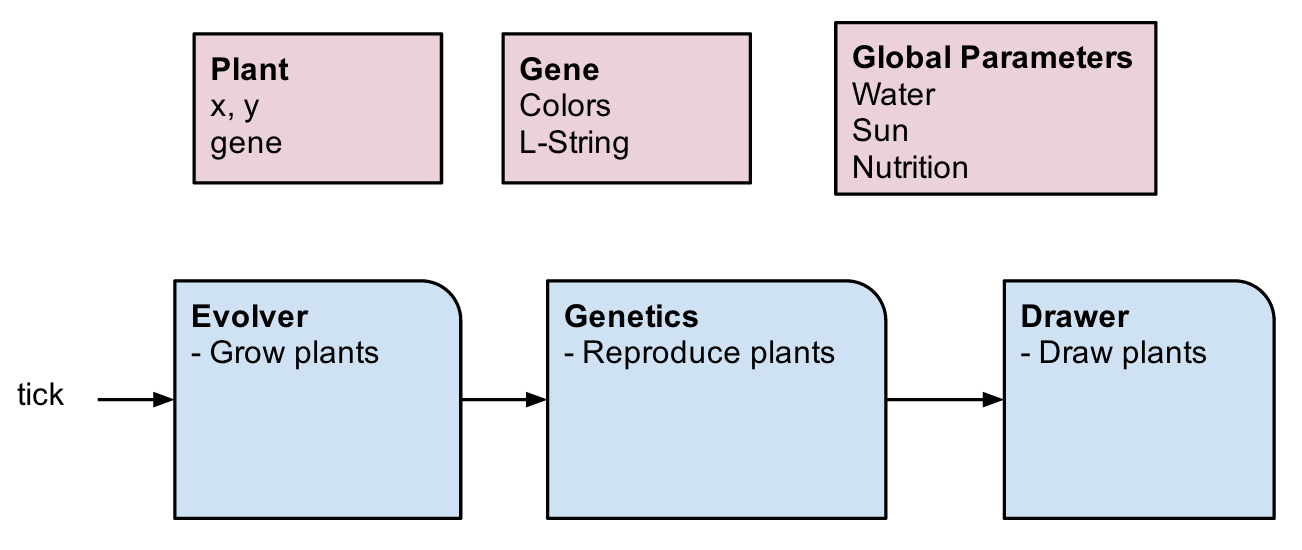
\includegraphics[width=\columnwidth]{images/architecture.png}

\section{Simulation}

The simulation of the plant environment is governed by ticks. For each tick that
goes, all plant objects becomes older. We wanted to have a realistic approach to
have plant grow in the real world, and therefore the first 4 ticks, the plant is
growing as a seed under ground. On the fifth tick it starts to grow above
ground. When the seventh tick is reached, the plant becomes mature and grows
flowers and leaves, if the gene is capable of it. The plant object then spreads
it seeds within a certain radius. When the season is over, the plant dies, but
it’s children grows up with either the same gene, or and mutation of the gene.

\section{Genetics}

In plant biology it’s defined two types of reproduction. Asexual reproduction
and sexual reproduction. Asexual reproduction can either be a clone or a
mutation of its parent. Sexual reproduction creates a new offspring by combining
the genetics from its parents.\cite{plantrepo}

\section{Conclusion}

Gene:

\begin{description}[leftmargin=!,labelindent=0.2in,labelwidth=0.1in]
  \item[F]   grow stem
  \item[L]   grow flower
  \item[X]   does not correspond to any drawing action and is used to control
             the evolution of the curve.\cite{lsystems}
  \item[n, e, s, w] \hfill \\
             bend plants growing direction either north, east, south or west.
             The angle is dependent on the genes angle.
  \item[{[}] push matrix
  \item[{]}] pop matrix
\end{description}

Example of a plant at first generation:

\begin{description}[leftmargin=!,labelindent=0.2in,labelwidth=0.4in]
  \item[Angle] 15 degrees
  \item[Axiom] X
  \item[Rules] \{ ``Fs[[F]eX]nF[wFX]F'' , ``FF'' \}
\end{description}

Notice that this plant will not start with flowers (`L').

Generally when the plant grows, it takes a random character from the LString
(but not `[' or `]') and substitutes this character with one random rule from
the plant gene. At the seventh tick of the season, the plant is mature and will
clone itself. There's two ways that this can happen. Either the new plant will
grow up with the same gene, or the gene will mutate and the new plant will be
given the mutated gene. The mutation happens in the set of the gene rules. A
random rule is picked out to be mutated. Again there is two possible outcomes.
Either a character in the rule will be deleted, or a random string from a
predefined mutation array will be added at a random position in the rule. We
want to simulate subtle changes in the gene as the mutation isn't suppose to be
extreme in any ways. Therefore the mutation array can be in the following way \{
``F'', ``L'', ``xF'', ``xL'', ``xX'', ``[X]'', ``[F]'', ``[L]'', ``[xF]'',
``[xL]'' \}. `x' is substituted with a random direction to grow, i.e. `n', `e',
`s' or `w'.

\section{Environmental parameters}

There are three basic environmental parameters which has an effect on the
plants. The amount of sun (0-100\%), water (0-100\%) and the nutrition available
in the ground. 

\section{Graphics}

\section{Conclusion}

%%%%%%%%%%%%%%
% References %
%%%%%%%%%%%%%%

\bibliographystyle{acmsiggraph}
\bibliography{paper}

\end{document}
